\documentclass[tikz,border=3.14mm]{standalone}
\usetikzlibrary{calc}
\begin{document}
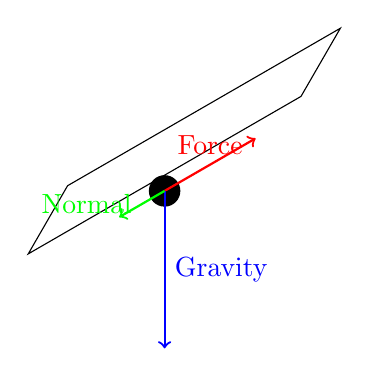
\begin{tikzpicture}

    % Define slope angle and length
    \def\angle{30}
    \def\length{4}

    % Draw incline
    \draw (0,0) -- (\angle:\length) -- ++ (90-\angle:1) -- ++(180+\angle:\length) -- cycle;

    % Draw object
    \coordinate (object) at ($(\angle:\length/2)+(0,-0.2)$);
    \fill (object) circle (0.2);

    % Draw forces
    \draw[thick, ->, red] (object) -- ++(\angle:\length/3) node[midway, above] {Force}; % Pulling force
    \draw[thick, ->, blue] (object) -- ++(-90:\length/2) node[midway, right] {Gravity}; % Gravitational force
    \draw[thick, ->, green] (object) -- ++(180+\angle:\length/6) node[midway, left] {Normal}; % Normal force

\end{tikzpicture}
\end{document}